\section{Dispositivos Ensaiados}
\label{sec:MetDispositivos}

Foram utilizadas as placas de desenvolvimento DE2 e ZedBoard. Elas foram escolhidas considerando suas disponibilidades no laboratório e por serem de fabricantes diferentes e possuírem nós tecnológicos diferentes.

A DE2 possui o FPGA EP2C35F672C6N da família o Cyclone II da fabricante Altera, pertencente a Intel, que possui um nó tecnológico de 90nm. A ZedBoard possui o SoC Zynq-7000, da Xilinx, agora pertencente a AMD, que contém um processardor ARM Cortex-A9 de dois núcleos e um FPGA Artix 7 de nó tecnológico de 28nm \cite{AmdFpga2}.

Ambas as placas possuem, além dos FPGAs, componentes e periféricos necessários para testes e prototipação de sistemas, como: botões, chaves, LEDs, display, memória flash e diversas entradas e saídas.

As Figuras \ref{fig:DE2Board} e \ref{fig:ZedBoard} mostram, respectivamente, a placa de desenvolvimento DE2 e ZedBoard utilizadas.

\begin{figure}[H]
    \centering
    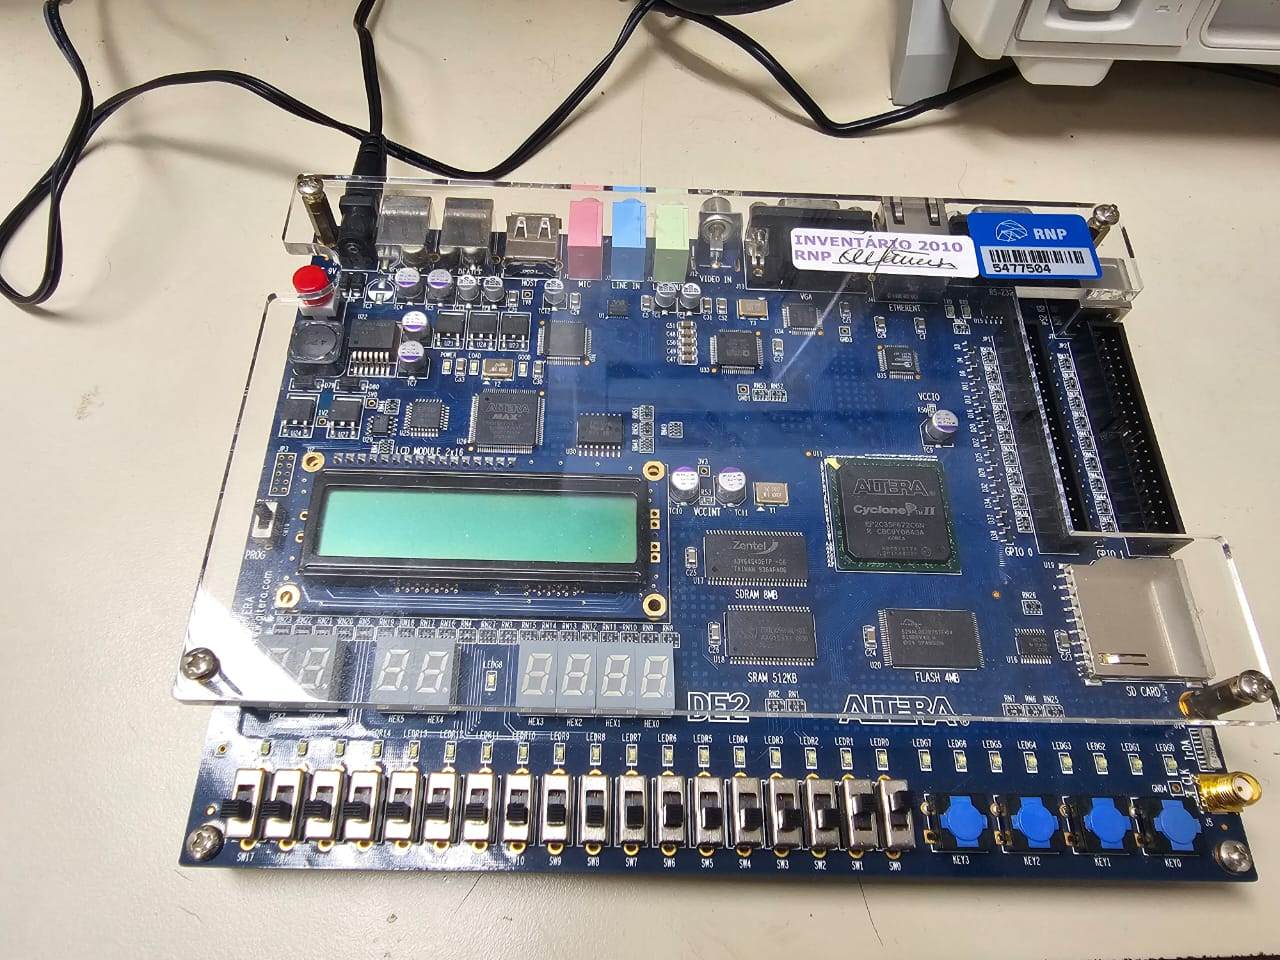
\includegraphics[scale=0.2]{figures/Metodologia/DE2.jpeg}
    \caption{Placa DE2. Fonte: O Autor}
    \label{fig:DE2Board}
\end{figure}

\begin{figure}[H]
    \centering
    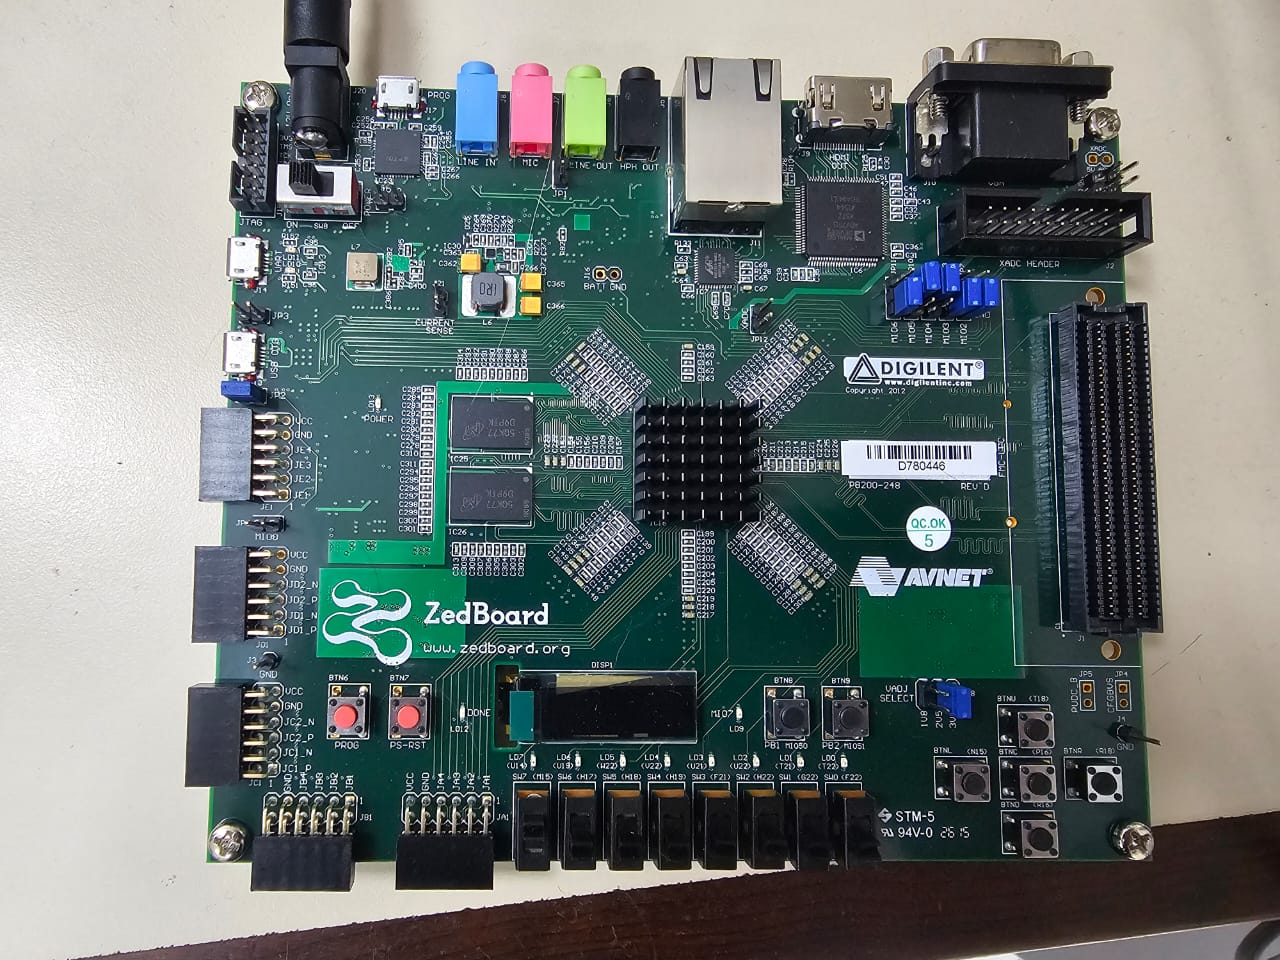
\includegraphics[scale=0.2]{figures/Metodologia/ZedBoard1.jpeg}
    \caption{Placa ZedBoard. Fonte: O Autor}
    \label{fig:ZedBoard}
\end{figure}

% EP2C35F672C6N K CBC9Y0843A
% https://community.element14.com/products/devtools/technicallibrary/w/documents/10126/altera-cyclone-fpga-series-overview

% The Zynq™ 7000 SoC family integrates the software programmability of an ARM®-based processor with the hardware programmability of an FPGA, enabling key analytics and hardware acceleration while integrating CPU, DSP, ASSP, and mixed signal functionality on a single device. Consisting of single-core Zynq 7000S and dual-core Zynq 7000 devices, the Zynq 7000 family offers an exceptional price to performance-per-watt, fully scalable SoC platform for your unique application requirements.
% Zynq 7000 devices are equipped with dual-core ARM Cortex-A9 processors integrated with 28nm Artix 7 or Kintex™ 7 based programmable logic for excellent performance-per-watt and maximum design flexibility. With up to 6.6M logic cells and offered with transceivers ranging from 6.25Gb/s to 12.5Gb/s, Zynq 7000 devices enable highly differentiated designs for a wide range of embedded applications including multi-camera drivers assistance systems and 4K2K Ultra-HDTV.
% https://www.xilinx.com/products/silicon-devices/soc/zynq-7000.html